\chapter[Itération~2:~(~3/8/2017~-~3/28/2017~)]{Itération~2:~\textup{\textto{(~3/8/2017~-~3/28/2017~)}}}

%\section*{Introduction}
%\addcontentsline{toc}{section}{Introduction}

Une caractéristique du Scrum est l'extension continue des spécifications du
produit élaboré dans l'itération précédente. En effet Scrum permet à s'adapter
au changement seulement entre les itérations. Dans ce contexte, les
fonctionnalités développées ont été étendues.

\section{But l'itération}

L'objectif de cette itération vise trois environnements. Nous allons ajouter
une nouvelle vision par rapport à l'itération précédentes.

Ils sont comme suites:

\begin{description}
    \item [Smartphone] L'ajout de nouvelles fonctionnalités comme:
        \begin{itemize}
            \item La capture de l'embouteillage.
            \item La détection des secousses.
            \item La déclaration des ralentisseurs.
        \end{itemize}
    \item [Dashboard] Enrichir la carte par:
        \begin{itemize}
            \item Des nouveaux marqueurs qui spécifient chaque type de rapport
                ajouté.
            \item Une légende pour le filtrage des marqueurs.
        \end{itemize}
    \item [Rapport] La création d'une page rapport qui permet à l'utilisateur
        de:
        \begin{itemize}
            \item Faire une description sur le type du rapport (violence,
                accident, déchet, \ldots)
            \item Charger une image.
            \item Choisir sa position automatiquement ou manuellement.
        \end{itemize}
\end{description}

%La méthodologie Scrum a eu un impact positif sur les développeurs, du point de
%vue social, elle a valorisé le travail en équipe, la solidarité, le respect et
%la communication entre toutes les parties prenantes (client, développeurs,
%\ldots). Elle a aussi changé leur vison sur le développement des logiciels.

%L'objectif de cette itération est d'ajouter un système de gestion des rapport,
%d'améliorer la qualité de service web de location et d'enrichir des
%fonctionnalités du \textquote{Dashboard}.

\section{Planification de l'itération}

Au sein de la réunion de planification nous avons sélectionné les tâches à
réaliser au cours de cette itération tout en accord avec le \textquote{Product
Owner}.

\subsection{Backlog de l'itération}

Le but de cette itération est d'ajouter un système de gestion des rapport,
d'améliorer la qualité et d'explorer des niveau type des donnes.

Le tableau~\ref{tab:sprint2-backlog} représente nos tâches dans cette itération.

\begin{center}
    \footnotesize
    \begin{longtable}{| p{1cm} | p{5cm} | p{7cm} | l |}
        \caption{Backlog de l'itération 2}
\label{tab:sprint2-backlog} \\

        \hline
        \multicolumn{1}{|c}{\textbf{Réf}} &
        \multicolumn{1}{|c}{\textbf{Spécification}} &
        \multicolumn{1}{|c}{\textbf{Description}} &
        \multicolumn{1}{|c|}{\textbf{P}} \\ \hline
        \endhead

        \hline \multicolumn{4}{|r|}{{Continué en page suivante$\dotsc$}} \\ \hline
        \endfoot

        \hline \hline
        \endlastfoot

        \hline
2.1 & Recherche sur les trajectoires & Comment présenter et enregistrer les trajectoire & 1 \\ \hline
2.2 & Affichage du trajet sur la carte & Visualizer le trajectoire d'un périphérique comme un ligne & 1 \\ \hline
2.3 & Implementer service d'enregistrement des ralentisseurs & Enregistrer les données nécessaires pour représenter un ralentisseur & 1 \\ \hline
2.4 & Responsive design & IHM de l'application Android adaptable aux différentes résolutions et rotations & 2 \\ \hline
2.5 & Implementer l'interface de déclaration un ralentisseur & Bouton rapport activé seulement si la localisation est active & 2 \\ \hline
2.6 & Filtrage des marqueurs dans la carte & Légende simplifiée permettant de choisir les types de données affichés dans la carte & 1 \\ \hline
2.7 & Implementer service de chargement de l'image & Charger, valider et enregistrer les images dans le serveur & 1 \\ \hline
2.8 & Implementer la fonctionnalité de déclaration des rapports & Formulaire avec validation et service d'enregistrement dans le serveur & 1 \\ \hline
2.9 & Recherche test unitaires & Comment améliorer la qualité du code et installation d'une solution des tests unitaires & 1 \\ \hline
2.10 & Recherche sur les frameworks PHP & Choisir le framework optimal pour notre platform et faire la migration & 2 \\ \hline
2.11 & Groupement de secousse sur la carte & Les marqueurs de secousses regroupés lors d'un zoom out sur la carte et séparer lors d'un zoom in & 3 \\ \hline
    \end{longtable}
\end{center}

\subsection{Estimation de l'itération}

Comme l'itération précédant, Nous avons fixé la période de cette itération à 3
semaine. Le budget horaire des membres est présenté dans le
tableau~\ref{tab:sprint2-capacity}.

\begin{table}[htbp]
    \centering
    \begin{tabular}{| c | c |}
        \hline
        \textbf{Membre} & \textbf{Budget Horaire} \\ \hline
        \hline
Moez & 144 \\ \hline
Rihab & 144 \\ \hline
\textbf{Total} & 288 \\ \hline
    \end{tabular}
    \caption{Budget horaire --- Itération 2}
\label{tab:sprint2-capacity}
\end{table}

Les estimations de nos tâches en heures sont disponibles dans le
tableau~\ref{tab:sprint2-estimation}.

\begin{center}
    \begin{longtable}{| l | l | l |}
        \caption{Nombre d'heures estimé pour la réalisation des tâches}
\label{tab:sprint2-estimation} \\

        \hline
        \multicolumn{1}{|c}{\textbf{Spécification}} &
        \multicolumn{1}{|c}{\textbf{Membre}} &
        \multicolumn{1}{|c|}{\textbf{Heures}} \\ \hline
        \endhead

        \hline \multicolumn{3}{|r|}{{Continué en page suivante$\dotsc$}} \\ \hline
        \endfoot

        \hline \hline
        \endlastfoot

        \hline
Recherche sur les trajectoires & Rihab & 5 $\times$ 2 \\ \hline
Affichage du trajet sur la carte & Moez & 13 $\times$ 2 \\ \hline
Implementer service d'enregistrement des ralentisseurs & Moez & 5 \\ \hline
Responsive design & Rihab & 5 $\times$ 2 \\ \hline
Implementer l'interface de déclaration d'un ralentisseur & Rihab & 13 $\times$ 2 \\ \hline
Filtrage des marqueurs dans la carte & Rihab & 13 \\ \hline
Implementer service de chargement de l'image & Moez & 5 \\ \hline
Implementer la fonctionnalité de déclaration des rapports & Moez & 5 \\ \hline
Recherche test unitaires & Moez & 5 \\ \hline
Recherche sur les frameworks PHP & Moez & 5 \\ \hline
Groupement de secousse sur la carte & Rihab & 5 \\ \hline
    \end{longtable}
\end{center}

%\subsubsection{Évolution du travail}

\section{Outils utilisés}

\subsection{Lumen}

On a décidé de migrer vers un framework pour le développement du backend du
notre plateforme dans le but de simplifier et améliorer nos services web. Les
critères de choisir le framework étaient sa performance, sa stabilité et son
support de développement des api RESTful. Les 3 frameworks principales étudiés:

\begin{description}
    \item [Slim] Un macro framework performant avec support de développement
        des services web de premiere classe. Il manque le support pour
        développer des sites web classiques.
    \item [Symfony] Le framework PHP de référence. Il suivre une architecture
        modulaire et fournit une haute performance. Pour ajouter le support des
        services web, il nécessite l'ajoute et configurations des multiples des
        extensions.
    \item [Lumen] Une version minimal du framework Laravel pour le
        développement des services web. Étant basé sur Laravel, il profile d'un
        excellent support des extensions du troisième partie.
\end{description}

Lumen était choisi pour sa simplicité de configurer et de lancer et pour son
support de migrer vers Laravel en cas ou on aura besoin de supporter le
développement du site web classique ou autres types de développement.


%Pour le développement de backend du notre plateforme, la langue du
%programmation PHP a été pré choisi. Mais, on avait la responsabilité de choisir
%les bibliothèques et les frameworks. Pendant la 1\iere{} itération, le but
%était de se familiariser avec la langue PHP\@. Donc, on a utilisé seulement les
%extensions officiel du PHP incluant PDO, \ldots. Dans l'itération suivante, on
%a étudié les frameworks disponibles. A la fin, on a choisi le framework Lumen
%qui est une version simplifié du Laravel pour le développement des API
%\acrshort{RESTful}.

\section{Mises des normes}

Outres que les critères de la premiere itération, les nouveaux critères à
respecter pour cette itération sont:

\subsection{Qualité du trajectoire}

Le trajectoire doit être aligné sur le trajet avec bonne précision. Et le
nombre des positions nécessaire pour tracer le trajectoire doivent être le
minimum le plus possible.

\subsection{Architecture modulaire}

Architecture de backend doit être modulaire: On doit changer notre code
procédurale par un code orienté objet et minimiser la duplication du code et
séparer le code des models et le code des contrôleurs.

\subsection{IHM de la page Dashboard Responsive}

Affiche claire et responsive des marqueurs dans la carte meme si le nombre est
très élevé.

\section{Conception}

La figure~\ref{fig:sprint2-webservices-report-usecase} synthétise le cas
d'utilisation du services \textquote{Rapport} de la deuxième itération.

\begin{figure}[htbp]
    \centering
    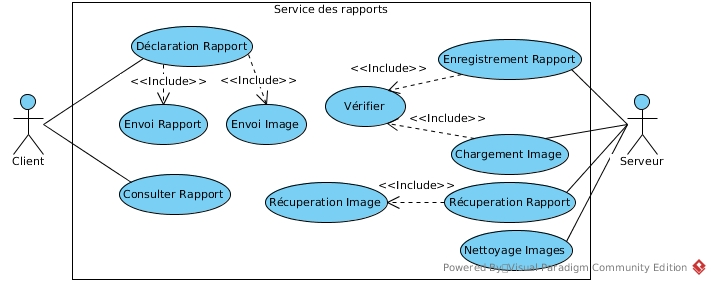
\includegraphics[width=1\textwidth]{sprint2-webservices-report-usecase}
    \caption{Diagramme de case d'utilisation du services Rapports --- Itération 2}
\label{fig:sprint2-webservices-report-usecase}
\end{figure}

Le schéma~\ref{fig:sprint2-webservices-class} présente le diagramme des classes
du service web dans cette itération.

\begin{figure}[htbp]
    \centering
    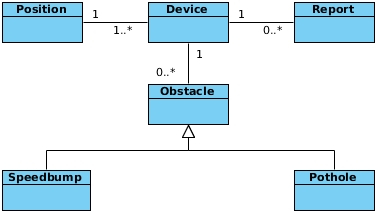
\includegraphics[width=0.8\textwidth]{sprint2-webservices-class}
    \caption{Diagramme de classe du service web --- Itération 2}
\label{fig:sprint2-webservices-class}
\end{figure}

Les deux
figures~\ref{fig:sprint2-webservices-report-post-sequence},~\ref{fig:sprint2-webservices-report-get-sequence}
décrit les scénarios de la mise à jour de la position dans la deuxième
itération.

\begin{figure}[htbp]
    \centering
    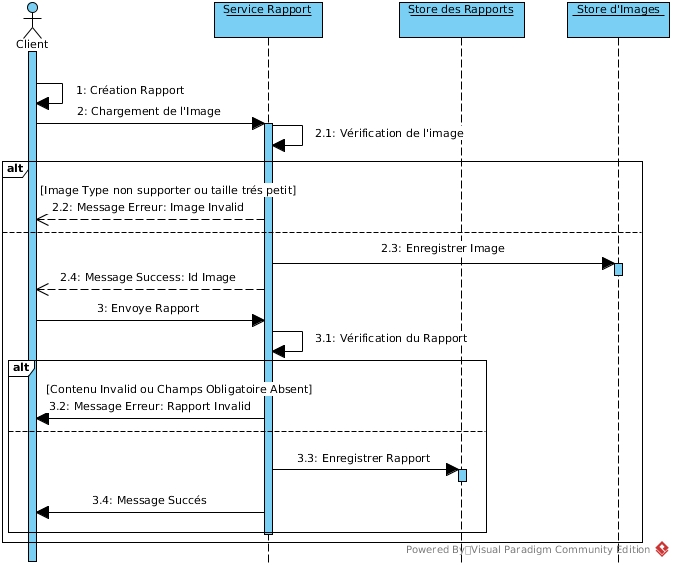
\includegraphics[width=1\textwidth]{sprint2-webservices-report-post-sequence}
    \caption{Diagramme de séquence du services Post Rapports --- Itération 2}
\label{fig:sprint2-webservices-report-post-sequence}
\end{figure}

\begin{figure}[htbp]
    \centering
    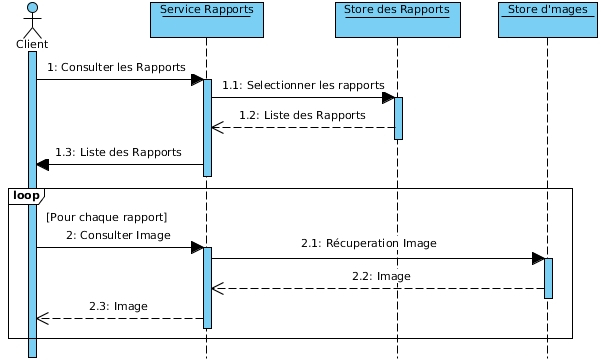
\includegraphics[width=1\textwidth]{sprint2-webservices-report-get-sequence}
    \caption{Diagramme de séquence du services Get Rapports --- Itération 2}
\label{fig:sprint2-webservices-report-get-sequence}
\end{figure}

La figure~\ref{fig:sprint2-dashboard-class} représente la nouvelle architecture
orienté objet de la page \textquote{Dashboard}.

\begin{figure}[htbp]
    \centering
    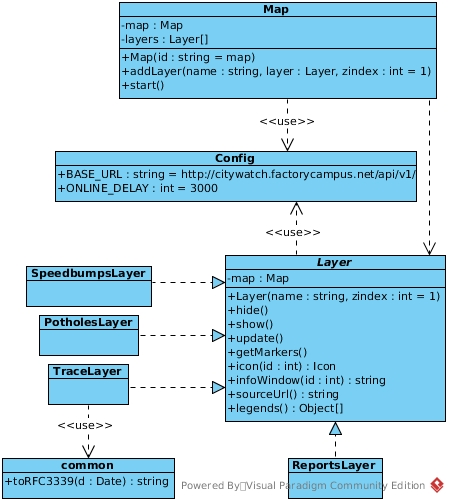
\includegraphics[width=0.9\textwidth]{sprint2-dashboard-class}
    \caption{Diagramme des classes du Dashboard --- Itération 2}
\label{fig:sprint2-dashboard-class}
\end{figure}

\section{Évaluation suivant les normes mises}

L'évaluation produite à la fin de la réunion de revue ne concerne que la satisfaction des clients
et si le produit est fonctionnel ou pas. Concernant ce sujet, des normes ont été mises afin d'évaluer
le prototype suivant les aspects de qualité, robustesse, \ldots.

\subsection{Contributions}

Au cours de l'itération avec l'augment des fonctionnalités ajoutées au
Dashboard, le code JavaScript devenu complexe, dupliqué et difficile à détecter
les bugs. On a décidé de réécrire le code avec une architecture modulaire et
plus moderne.

L'utilisation de la version ECMAScript 6 du JavaScript nous a fourni les
techniques de base nécessaires comme POO, Template Strings, paramètres par
défaut, nouvelles variantes de la boucle For et support de la programmation
asynchrone.

La nouvelle architecture est décrite dans le
diagram~\ref{fig:sprint2-dashboard-class}. Elle consiste de:

\begin{itemize}
    \item Une classe \verb|Map| contenu tout le logique métier d'initialiser et
        afficher la carte, registre et filtrer des différents types de données
        et traiter les différents évènements d'interaction humaine machine.
    \item Une classe abstract \verb|Layer| contenu tout le logique relié à
        chaque types des données à visualiser dans la map (téléchargement
        continuellement les données, génération les marqueurs ou zones, mise à
        jour des données, définition des filtrages supportés et les
        informations additionnelles à afficher). Le code commun entre
        différents layers est implémenté dans cette classe abstract.
    \item Une classe pour chaque type de données à visualiser (trajectoire,
        ralentisseurs, secousses, \ldots) qui hérite du classe \verb|Layer|. La
        plupart du temps, on a juste besoin de définir l'URL du resource, la
        listes des icons et des filtrages possibles.
    \item Un espace de noms \verb|Config| contenu les constantes de
        configuration.
\end{itemize}

\section{Revue de cette itération}


Dés que le temps de l'itération finisse, l'équipe organise une réunion de revue dans
le but d'évaluer le prototype développé.

\subsection{Produit de l'itération}

A la fin de l'itération 2, nous détaillons les différentes spécifications qui
caractérisent et implémenté le système de gestion des rapport.

\subsubsection{Page \textquote{Rapport}}

Dans cette page, nous donne la main à l'utilisateur pour faire un petit rapport
comme expliqué dans la figure~\ref{fig:sprint2-rapport-screenshot1}. Cette page
permet à l'utilisateur d'envoyer son rapport au serveur pour l'enregistrer. La
position du rapport est détecté automatique à travers l'api JavaScript standard
Location. On donne la main à l'utilisateur pour changer la location
manuellement en glissant le marqueur ou en changer les inputs. Le chargement de
l'image est obligatoire.

\TODO{Cette obligation était éliminer en review}

L'envoie du rapport est éxecuté en deux phases:

\begin{enumerate}
    \item Chargement de l'image au serveur. Si le type et le taille de l'image
        est valide, le serveur retourne un id unique (UUID) de l'image.
    \item Envoie du rapport au serveur. Les informations envoyées sont: type du
        rapport, id image, commentaire (optionnel) et les coordonnées.
\end{enumerate}

\begin{figure}[htbp]
    \centering
    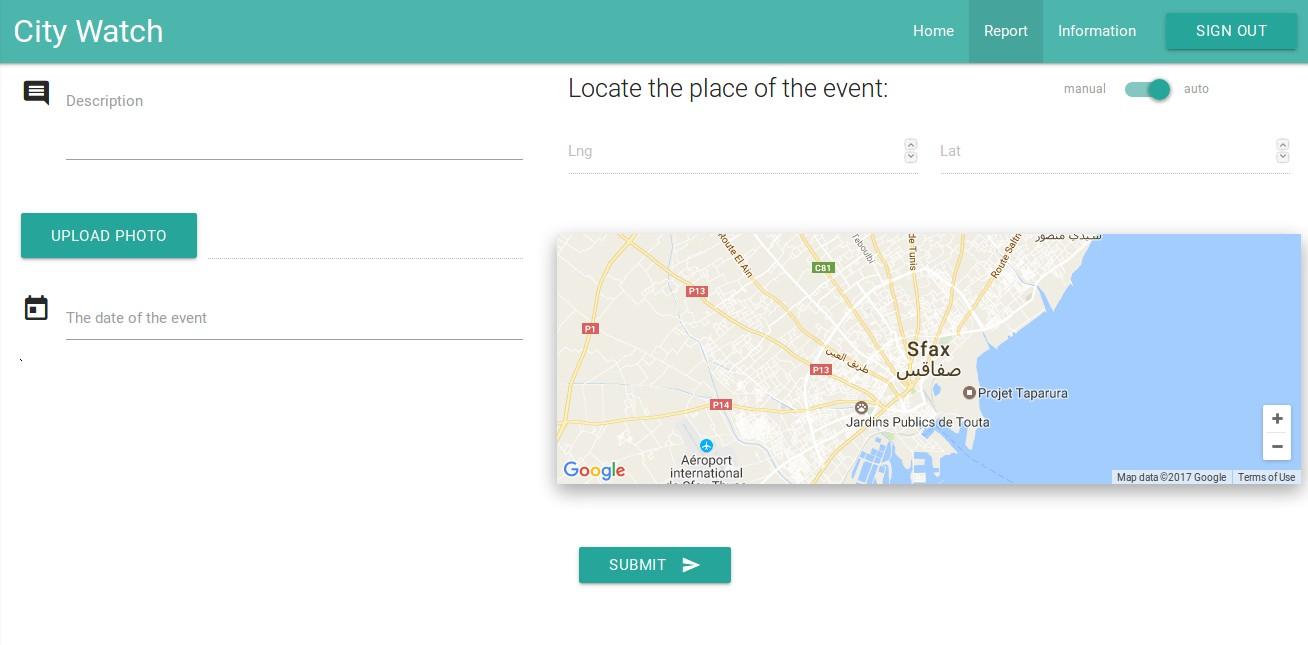
\includegraphics[width=0.7\textwidth]{sprint2-rapport-screenshot1}
    \caption{Page Rapport}
\label{fig:sprint2-rapport-screenshot1}
\end{figure}

\subsubsection{Page \textquote{Dashboard}}

L'utilitaire de regroupement de marqueurs vous aide à gérer plusieurs marqueurs
à différents niveaux de zoom. Précisément, les marqueurs sont en fait des
éléments à ce stade et ne deviennent réellement des marqueurs qu'après leur
rendu. Par souci de clarté, nous ne parlerons que de marqueurs dans ce
document.

Lorsqu'un utilisateur affiche la carte à un niveau de zoom élevé comme montre
la figure~\ref{fig:sprint2-dashboard-screenshot1}, les différents marqueurs
s'affichent sur la carte. Lorsqu'il effectue un zoom arrière comme montre la
figure~\ref{fig:sprint2-dashboard-screenshot2}, les marqueurs se regroupent
pour faciliter la consultation de la carte.

\begin{figure}[htbp]
    \begin{subfigure}{.5\textwidth}
        \centering
        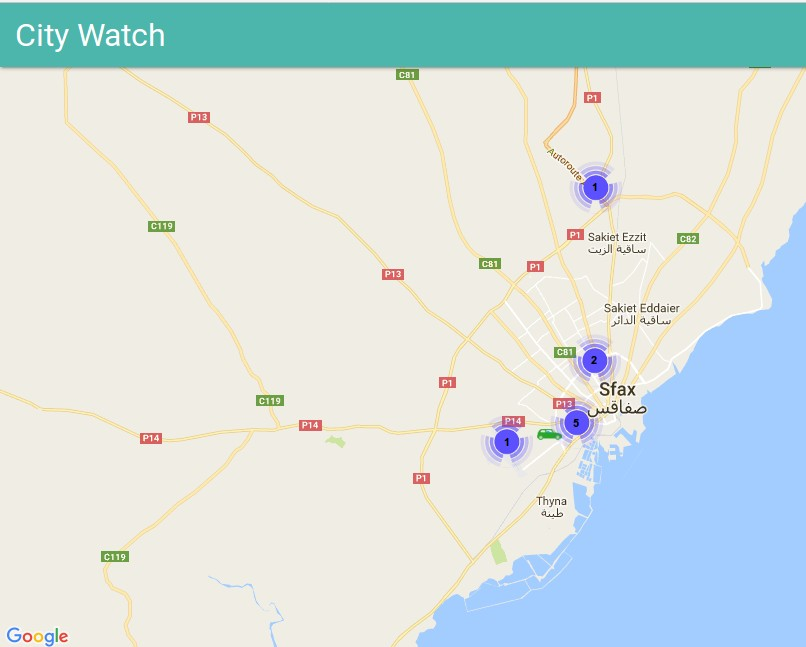
\includegraphics[width=.9\linewidth]{sprint2-dashboard-screenshot1}
        \caption{Groupement activé en un zoom bas}
\label{fig:sprint2-dashboard-screenshot1}
    \end{subfigure}
    \begin{subfigure}{.5\textwidth}
        \centering
        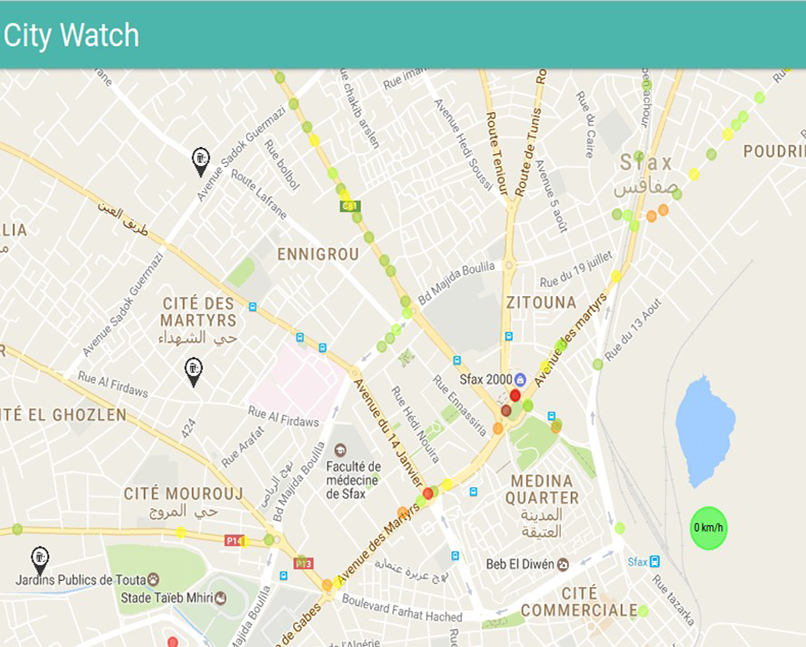
\includegraphics[width=.9\linewidth]{sprint2-dashboard-screenshot2}
        \caption{Groupement désactivé en zoom haut}
\label{fig:sprint2-dashboard-screenshot2}
    \end{subfigure}
    \caption{Groupement des secousses en différents niveaux du zoom}
\end{figure}

\subsubsection{Application Mobile \textquote{CityWatch}}

Dans notre application, l'utilisateur doit s'inscrit pour accéder à
l'application. Les données saisies dans le formulaire d'inscription (nom
d'utilisation, mot de passe) seront envoyées et stockées en toute sécurité et
confidentialité. Lorsqu'un utilisateur tend à se connecter, il tape son mot de
passe déjà saisies dans le formulaire d'inscription, alors une vérification
avec le serveur doit avoir lieu.

\textbf{Note:} Pour chaque nom d'utilisateur ajouté, le serveur vérifie
l'unicité de ce dernier.

\begin{figure}[htbp]
\centering
    \begin{subfigure}{.45\textwidth}
        \centering
        \centering
        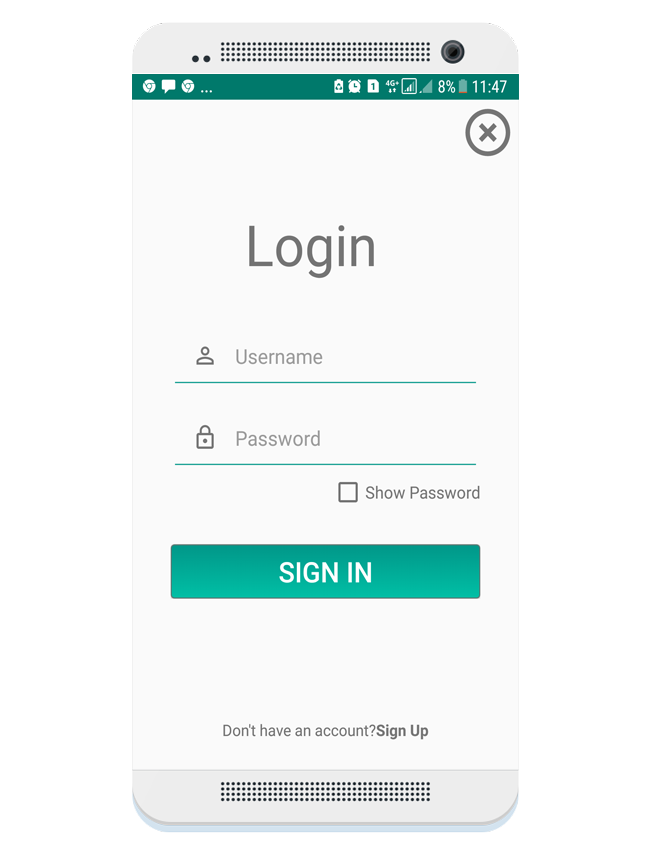
\includegraphics[width=1.0\linewidth]{sprint2-android-screenshot1}
        \caption{Activité du confection}
\label{fig:sprint2-android-screenshot1}
    \end{subfigure}
    \begin{subfigure}{.45\textwidth}
        \centering
        \centering
        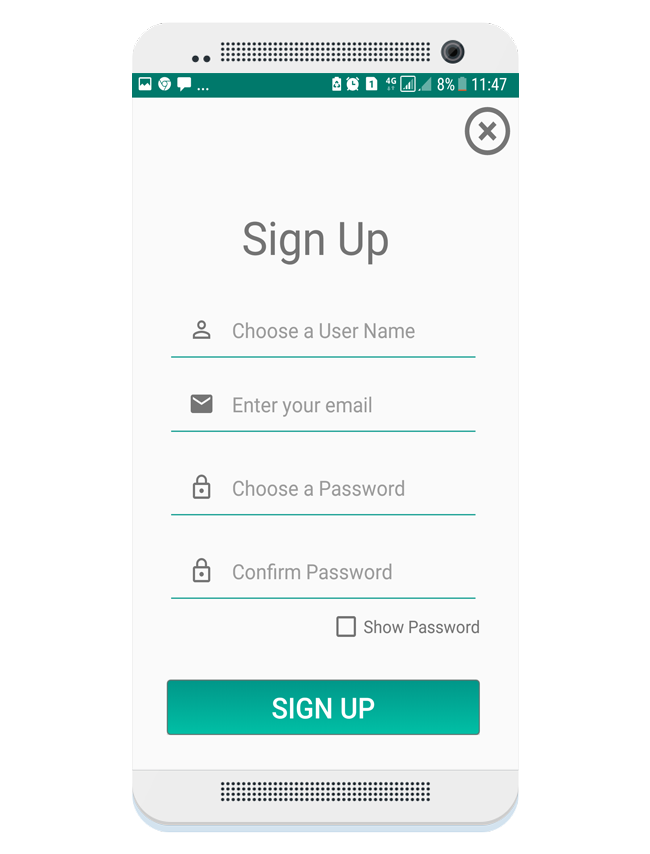
\includegraphics[width=1.0\linewidth]{sprint2-android-screenshot2}
        \caption{Activité d'inscription}
\label{fig:sprint2-android-screenshot2}
    \end{subfigure}
    \caption{Formulaire d'inscription}
\end{figure}

\subsection{Avis du Product Owner}

A la fin de cette deuxième itération, nous avons présenté au \textquote{Product
Owner} le produit obtenu. Le \textquote{Product Owner} a exprimé sa
satisfaction du travail réalisé et nous a conseillé par la suite de simplifier
le formulaire du rapport.

\subsection{Burndown chart}

La figure~\ref{fig:sprint2-burndown} présente une vue d'ensemble sur le progrès
de notre travail au cours de l'itération par rapport au progrès idéal.

\usetikzlibrary{plotmarks}

\begin{figure}
\centering
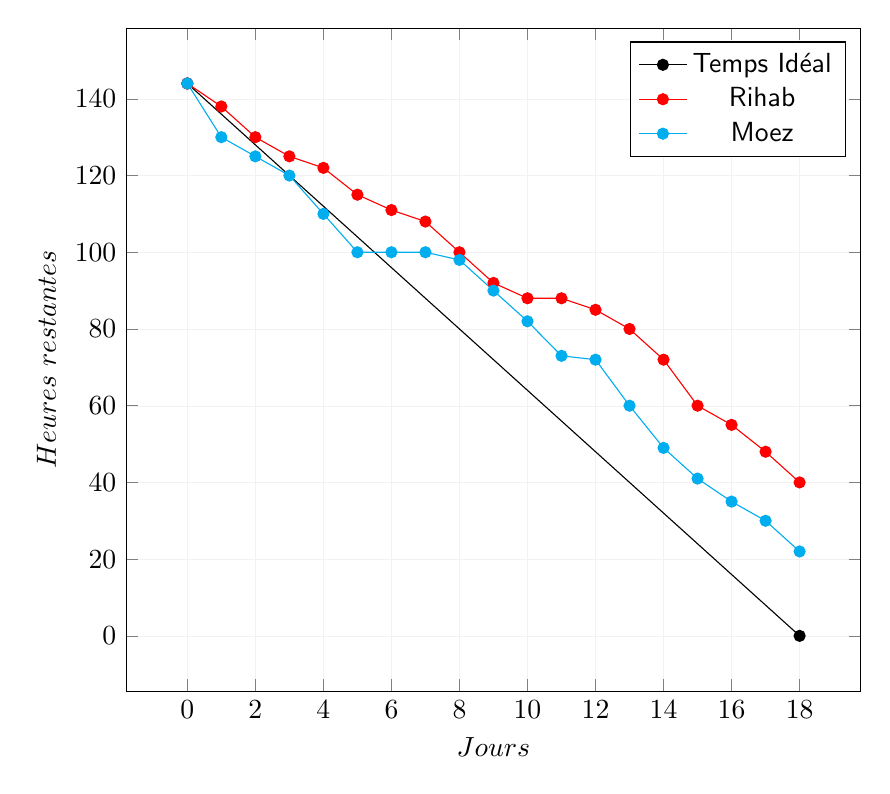
\begin{tikzpicture}[y=.1cm, x=.7cm,font=\sffamily]
\begin{axis}[
xlabel=$Jours$,
ylabel=$Heures\ restantes$,
grid=both,
grid style={line width=.1pt, draw=gray!10},
width=0.9\textwidth,
height=10cm,
%major grid style={line width=.2pt,draw=gray!50},
]
\addplot[color=black,mark=*] coordinates {
        (0,144)
        (18,0)
    };
    \addlegendentry{Temps Idéal}

    \addplot[mark=*,red] plot coordinates {
        (0, 144)
        (1, 138)
        (2, 130)
        (3, 125)
        (4, 122)
        (5, 115)
        (6, 111)
        (7, 108)
        (8, 100)
        (9, 92)
        (10, 88)
        (11, 88)
        (12, 85)
        (13, 80)
        (14, 72)
        (15, 60)
        (16, 55)
        (17, 48)
        (18, 40)
       
    };
    \addlegendentry{Rihab}
      \addplot[mark=*,cyan] plot coordinates {
        (0, 144)
        (1, 130)
        (2, 125)
        (3, 120)
        (4, 110)
        (5, 100)
        (6, 100)
        (7, 100)
        (8, 98)
        (9, 90)
        (10, 82)
        (11, 73)
        (12, 72)
        (13, 60)
        (14, 49)
        (15, 41)
        (16, 35)
        (17, 30)
        (18, 22)
       
    };
    \addlegendentry{Moez}
\end{axis}
\end{tikzpicture}
\caption{Graphique d'avancement - Itération 2}
\end{figure}


\section*{Conclusion}
\addcontentsline{toc}{section}{Conclusion}

Dans cette itération, la qualité de notre code a été bien améliorée grâce aux
testes unitaires que nous avons pris et le revue collaboré du code à chaque
changement. De plus l'utilisation d'un framework dans le développement de
notre service web a facilité et organisé notre code.

Le tableau~\ref{tab:sprint2-evaluation} présente le pourcentage de
réalisation de nos tâches de cette itération.
\begin{center}
    \begin{longtable}{| l | l |}
        \caption{Liste des tâches réalisées de deuxième itération}
\label{tab:sprint2-evaluation} \\

        \hline
        \textbf{Les tâches} & \textbf{Taux de réalisation} \\ \hline
        \endhead

        \hline \multicolumn{2}{|r|}{{Continué en page suivante$\dotsc$}} \\ \hline
        \endfoot

        \hline \hline
        \endlastfoot

        \hline
Recherche sur les trajectoires & Effectué 100\% \\ \hline
Affichage du trajet sur la carte & Effectué 100\% \\ \hline
Implementer service d'enregistrement des ralentisseurs & Effectué 100\% \\ \hline
Responsive design & Effectué 80\% \\ \hline
Implementer l'interface de déclaration d'un ralentisseur & Effectué 100\% \\ \hline
Filtrage des marqueurs dans la carte & Effectué 100\% \\ \hline
Implementer service de chargement de l'image & Effectué 70\% \\ \hline
Implementer la fonctionnalité de déclaration des rapports & Effectué 100\% \\ \hline
Recherche test unitaires & Effectué 80\% \\ \hline
Recherche sur les frameworks PHP & Effectué 100\% \\ \hline
Groupement de secousse sur la carte & Effectué 100\% \\ \hline
    \end{longtable}
\end{center}
